% Compile twice with pdflatex (or once with tectonic). Figures in figures/ are copies of ../figures.
% Schedule: 10 minutes + 5 minutes viva/demo. 10 main slides + 3 backup slides.
% Sumedh Navuda presents slides 1-5, Aldino presents slides 6-10 (about 5 minutes each).
\documentclass[aspectratio=169,11pt]{beamer}
\usetheme{Warsaw}
\usecolortheme{default}
\usepackage[T1]{fontenc}
\usepackage{lmodern,amsmath,booktabs,tabularx}
\definecolor{afgml}{RGB}{22,57,86}
\setbeamercolor{structure}{fg=afgml}
\setbeamertemplate{navigation symbols}{}
\setbeamertemplate{footline}[frame number]
\newif\ifguidance\guidancefalse
\newcommand{\help}[1]{\ifguidance\begin{block}{Preparation guidance}\small #1\end{block}\fi}
\newcommand{\fillin}[1]{[\textit{#1}]}
% Team facts used by every document in writeup/, report/ and slides/. Edit here once.
\newcommand{\StudentA}{Sumedh Navuda}
\newcommand{\StudentB}{Aldino}
\newcommand{\Authors}{\StudentA{} and \StudentB{}}
\newcommand{\Contact}{sumedhnavuda@outlook.com}
\newcommand{\RollA}{[roll no.]}   % <- replace with Sumedh's roll number
\newcommand{\RollB}{[roll no.]}   % <- replace with Aldino's roll number
\newcommand{\RepoURL}{https://github.com/sumedhnvda/ict5143-p8-fairness-audits}
\newcommand{\TeamID}{[team ID]}   % <- replace with the team ID given by the instructor
\newcommand{\SubmitTag}{submission-v1}

\graphicspath{{figures/}}
\newcommand{\good}[1]{\textcolor{green!45!black}{\textbf{#1}}}
\newcommand{\bad}[1]{\textcolor{red!70!black}{\textbf{#1}}}
\title[AFGML Capstone]{When Does Pooling Make Intersectional\\Fairness Audits Falsely Reassuring?}
\subtitle{ICT 5143: AFGML Capstone | Problem 8: Reliable intersectional fairness audits}
\author{\StudentA{} (\RollA) \and \StudentB{} (\RollB)}
\date{Team \TeamID{} \quad\textperiodcentered\quad \url{\RepoURL}}
\begin{document}
% ---------------------------------------------------------------- Sumedh Navuda: slides 1-5
% Slide 1: 20 seconds. Sumedh introduces team and question.
\begin{frame}\titlepage\end{frame}

% Slide 2: 50 seconds.
\begin{frame}{Research question and decision context}
\begin{itemize}
\item \textbf{Context:} an agency can contact only 30\% of a list with \emph{hypothetical} information outreach about
  public coverage. A Bayesian network ranks people; the top 30\% are contacted.
\item \textbf{Stakeholders:} people without public coverage who are never contacted, often in small
  race$\times$sex$\times$disability groups; the auditor who must sign off on the rule.
\item $Y=1$: \textbf{no public coverage} in the ACS record (not ``uninsured'', not ``eligible'').
  $D=1$: selected for outreach.
\item \textbf{Question:} when does hierarchical pooling make an audit say
  $\Delta\text{EOpp}=\max_g\text{TPR}_g-\min_g\text{TPR}_g\le0.10$ when the rule is unfair?
\item \textbf{H1:} when $\lambda$ is chosen on validation and a pooled audit certifies $\le0.10$, the frozen rule
  exceeds 0.10 on test in \textbf{more than half} of cases. Refuted if at most half fail on Texas.
\end{itemize}
\end{frame}

% Slide 3: 50 seconds.
\begin{frame}{Closest work and proposed contribution}
\begin{itemize}
\item \textbf{Established:} Bayesian hierarchical estimation of intersectional fairness (Foulds et al., SDM 2020);
  structured regression for tiny subgroups (Herlihy et al., FAccT 2024); $\epsilon$-contamination priors
  (Berger \& Berliner 1986); marginal fairness can hide subgroup unfairness (Kearns et al., ICML 2018).
\item \textbf{Open issue:} whether pooled \emph{audit criteria} produce false ``gap $\le\epsilon$'' claims when
  used to choose a decision rule on a real sparse design. We found no paper that tests this.
\item \textbf{Contribution:} (i) a controlled evaluation of when pooling masks sparse disparities (H1);
  (ii) a fix: \textbf{design-matched calibration} plus \textbf{held-out certification} (H2a--c).
  We claim no new prior and no new metric.
\item \textbf{Evidence needed:} out-of-sample Texas test of H1; paired $\Delta J$ against every established audit;
  an ablation without design matching and without held-out certification.
\end{itemize}
{\footnotesize 19-paper comparison table: \texttt{writeup/literature\_review.pdf}}
\end{frame}

% Slide 4: 60 seconds.
\begin{frame}{Data and evaluation population}
\begin{columns}[T]
\begin{column}{0.55\textwidth}
\begin{itemize}
\item Folktables ACSPublicCoverage, ACS PUMS 2018 1-year; CA core, TX replication.
\item Filter AGEP $<65$, PINCP $\le30{,}000$: \textbf{138,554} people, \textbf{85,182} households; $P(Y{=}1)=0.631$.
\item Protected: recorded race (9 codes), sex, disability $\Rightarrow$ 36 intersections.
\item Split 60/20/20 \textbf{by household} (SERIALNO), 5 seeds. Features: the 19 Folktables inputs.
\item Small groups: only \textbf{21 of 35} test intersections have $\ge30$ positives; the rest are exploratory.
\end{itemize}
\end{column}
\begin{column}{0.42\textwidth}
\footnotesize Same BN decisions, seed 0 test:\\[2pt]\setlength{\tabcolsep}{4pt}
\begin{tabular}{lcc}\toprule
Grouping & groups ($\ge$30) & $\Delta$EOpp\\\midrule
Sex & 2 (2) & 0.162\\
Disability & 2 (2) & 0.384\\
Race & 9 (8) & 0.597\\
Sex$\times$Dis & 4 (4) & 0.468\\
Race$\times$Sex$\times$Dis & 35 (21) & \bad{0.746}\\\bottomrule
\end{tabular}\\[4pt]
Intersections expose a gap that one attribute hides (Experiment 1).
\end{column}
\end{columns}
\end{frame}

% Slide 5: 90 seconds. Sumedh completes the first half.
\begin{frame}{Graphical model and inference}
\begin{columns}[T]
\begin{column}{0.52\textwidth}
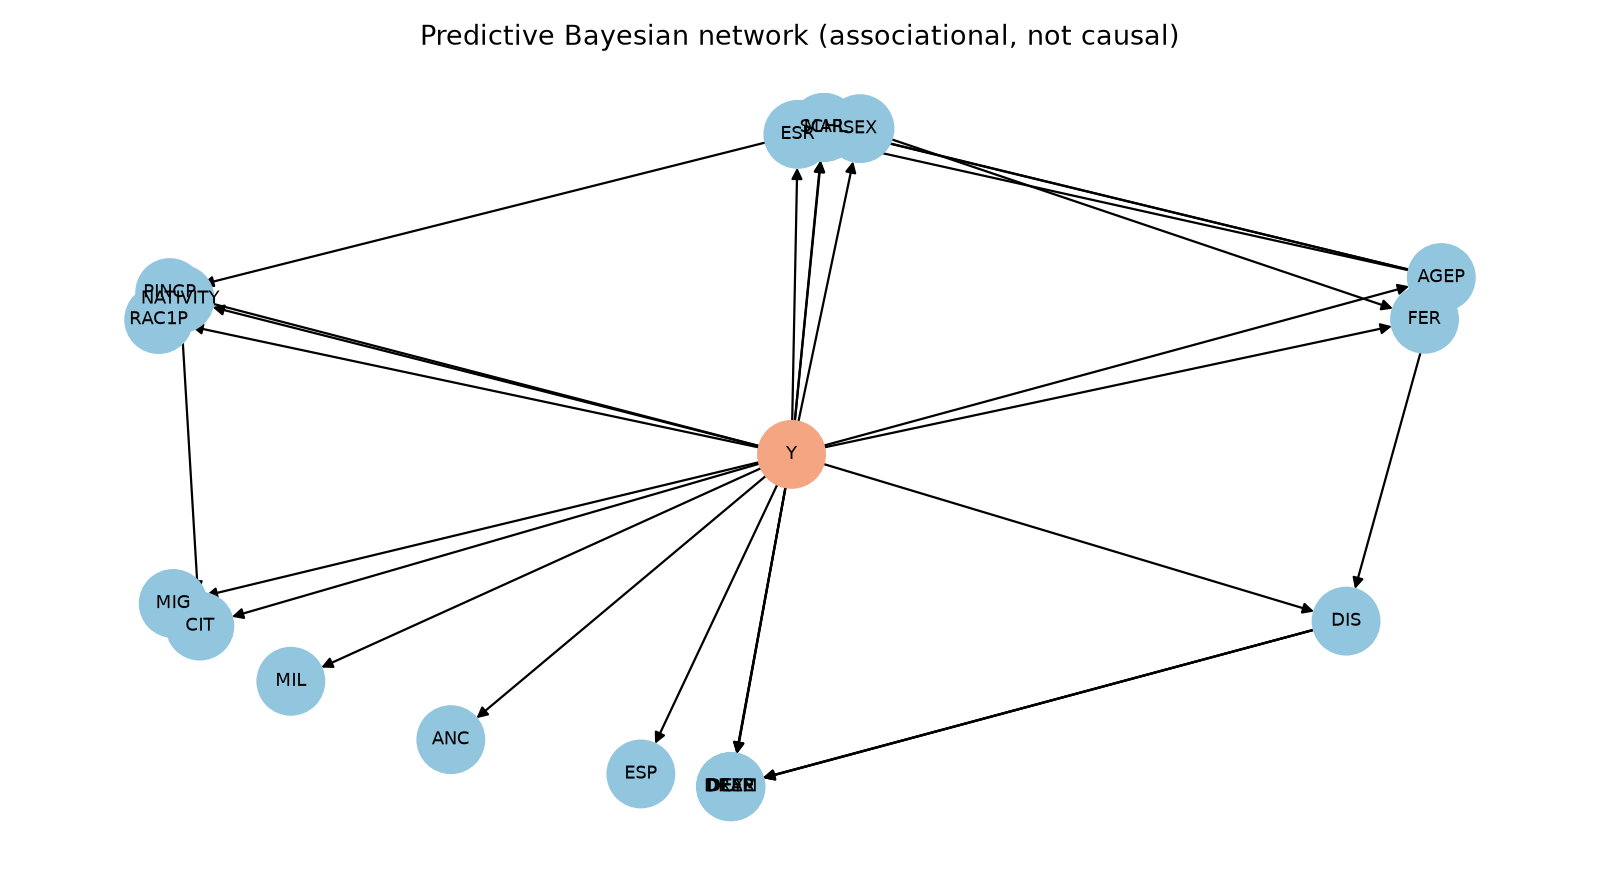
\includegraphics[width=\linewidth]{bn_structure}
\end{column}
\begin{column}{0.46\textwidth}
\footnotesize
\[p(y,\mathbf{x})=p(y)\textstyle\prod_j p(x_j\mid \mathrm{pa}(x_j))\]
\begin{itemize}
\item Augmented naive Bayes: $Y\to$ all 18 features, plus 10 feature edges (e.g.\ DIS$\mid$AGEP); Dirichlet
  $\alpha=1$ CPTs. \textbf{Associational, not causal.}
\item Query $P(Y{=}1\mid\mathbf{x}_E)$ by exact variable elimination; held-out codes clipped to the training range.
\item Validation: our VE (2 orders), pgmpy VE, clique tree and enumeration agree to $\mathbf{3.3\times10^{-16}}$ over 200
  evidence masks (tolerance $10^{-9}$); joint CI $\text{SEX}\perp\{\text{AGEP},\text{DIS}\}\mid Y$ checked.
\item Test AUROC 0.729 (LR 0.716, GBT 0.768).
\end{itemize}
\end{column}
\end{columns}
\end{frame}

% ---------------------------------------------------------------- Aldino: slides 6-10
% Slide 6: 60 seconds. Aldino starts.
\begin{frame}{Fairness criterion and proposed method}
\begin{itemize}
\item \textbf{Primary criterion:} intersectional equal opportunity (TPR range). The harm is missing people who need outreach.
\item \textbf{Utility:} recall at 30\% capacity; allowed loss $\le0.02$ (preregistered).
\item \textbf{Audit model:} $k_g\sim\text{Bin}(n_g,\theta_g)$ for selected positives. Comparators: raw, independent Beta, complete,
  exchangeable EB / full Bayes, \texttt{struct} (logit main effects $+\,u_g$, $u_g\sim N(0,\tau^2)$).
\item \textbf{Proposed:} contamination prior $\theta_g\sim\pi\,\text{Beta}(a,b)+(1-\pi)\,\text{slab}$, with $\pi_{\max}$,
  slab and rule chosen by $\max J=\text{ACC}-\overline{\text{FTS}}$ on worlds built on the \textbf{target state's
  validation group sizes}. Then choose $\lambda$ on validation half A and \textbf{certify on half B}.
\item \textbf{$A$ at prediction time:} yes. The scores use race, sex and disability; for $\lambda>0$ so do the thresholds.
\item \textbf{Diagnostics:} $\Delta$DP, $\Delta$EOdds, selection ratio, worst-group recall, group ECE, PPC, interval coverage.
\end{itemize}
\end{frame}

% Slide 7: 60 seconds.
\begin{frame}{Experimental protocol}
\begin{itemize}
\item \textbf{Baselines:} LR, GBT (predictive); BN without uncertainty-aware selection (graphical); raw, independent,
  complete, hier EB, full Bayes, \texttt{struct} audits (fairness).
\item \textbf{Matched:} same counts for every audit; same capacity (matched on validation); same rule family $R(\lambda)$,
  $\lambda\in\{0,0.1,\dots,1\}$.
\item \textbf{Selection:} train fits edges and CPTs; validation picks thresholds and $\lambda$; test only evaluates frozen rules.
  Calibration of the audit uses simulated outcomes only.
\item \textbf{Runs and intervals:} 5 household splits; household-cluster Poisson bootstrap B\,=\,1000, Holm over 2
  confirmatory comparisons; paired $\Delta J$ bootstrap over simulated worlds (B\,=\,2000).
\item \textbf{Mechanism tests:} E1--E5, minority thinning (1, 0.5, 0.25, 0.1), semi-synthetic deficit worlds (cell,
  interaction, disability main effect), prior/tolerance grids, survey weights, Texas replication.
\end{itemize}
\end{frame}

% Slide 8: 90 seconds.
\begin{frame}{Main result and uncertainty}
\begin{columns}[T]
\begin{column}{0.5\textwidth}
\footnotesize Fresh Texas worlds (200 per cell), $\epsilon=0.10$\\[2pt]
\begin{tabular}{lccc}\toprule
Audit & ACC$\uparrow$ & FTS$\downarrow$ & $J\uparrow$\\\midrule
Full Bayes, plug-in & 1.000 & 0.615 & 0.385\\
Hier EB, upper 0.9 & 0.985 & 0.625 & 0.360\\
\texttt{struct}, plug-in & 0.108 & 0.073 & 0.034\\
\textbf{Design-matched} & 0.832 & 0.168 & \good{0.664}\\\bottomrule
\end{tabular}\\[6pt]
\begin{tabular}{lcc}\toprule
Real CA+TX (10 splits) & claims & false\\\midrule
Same-data certification & 10 & \bad{10}\\
\textbf{Held-out certification} & 0 & \good{0}\\\bottomrule
\end{tabular}\\[2pt]
Mean test recall 0.365 in both.
\end{column}
\begin{column}{0.48\textwidth}
\textbf{Paired $\Delta J$ (95\% CI):}\\
vs best established: \good{$+0.279$ [0.235, 0.322]}\\
vs earlier calibration: $+0.475$ [0.422, 0.525]\\[6pt]
\textbf{H1:} 116/116 CA and \textbf{27/27} TX pooled validation claims failed on test $\Rightarrow$ supported.\\[6pt]
\textbf{Answer:} pooled ``gap $\le0.10$'' claims are not trustworthy for sparse intersections. Calibrating on the
real design and certifying on held-out households gives the best audit out of sample on Texas; on California it ties.
\end{column}
\end{columns}
\end{frame}

% Slide 9: 60 seconds.
\begin{frame}{Ablation, robustness and failure case}
\centering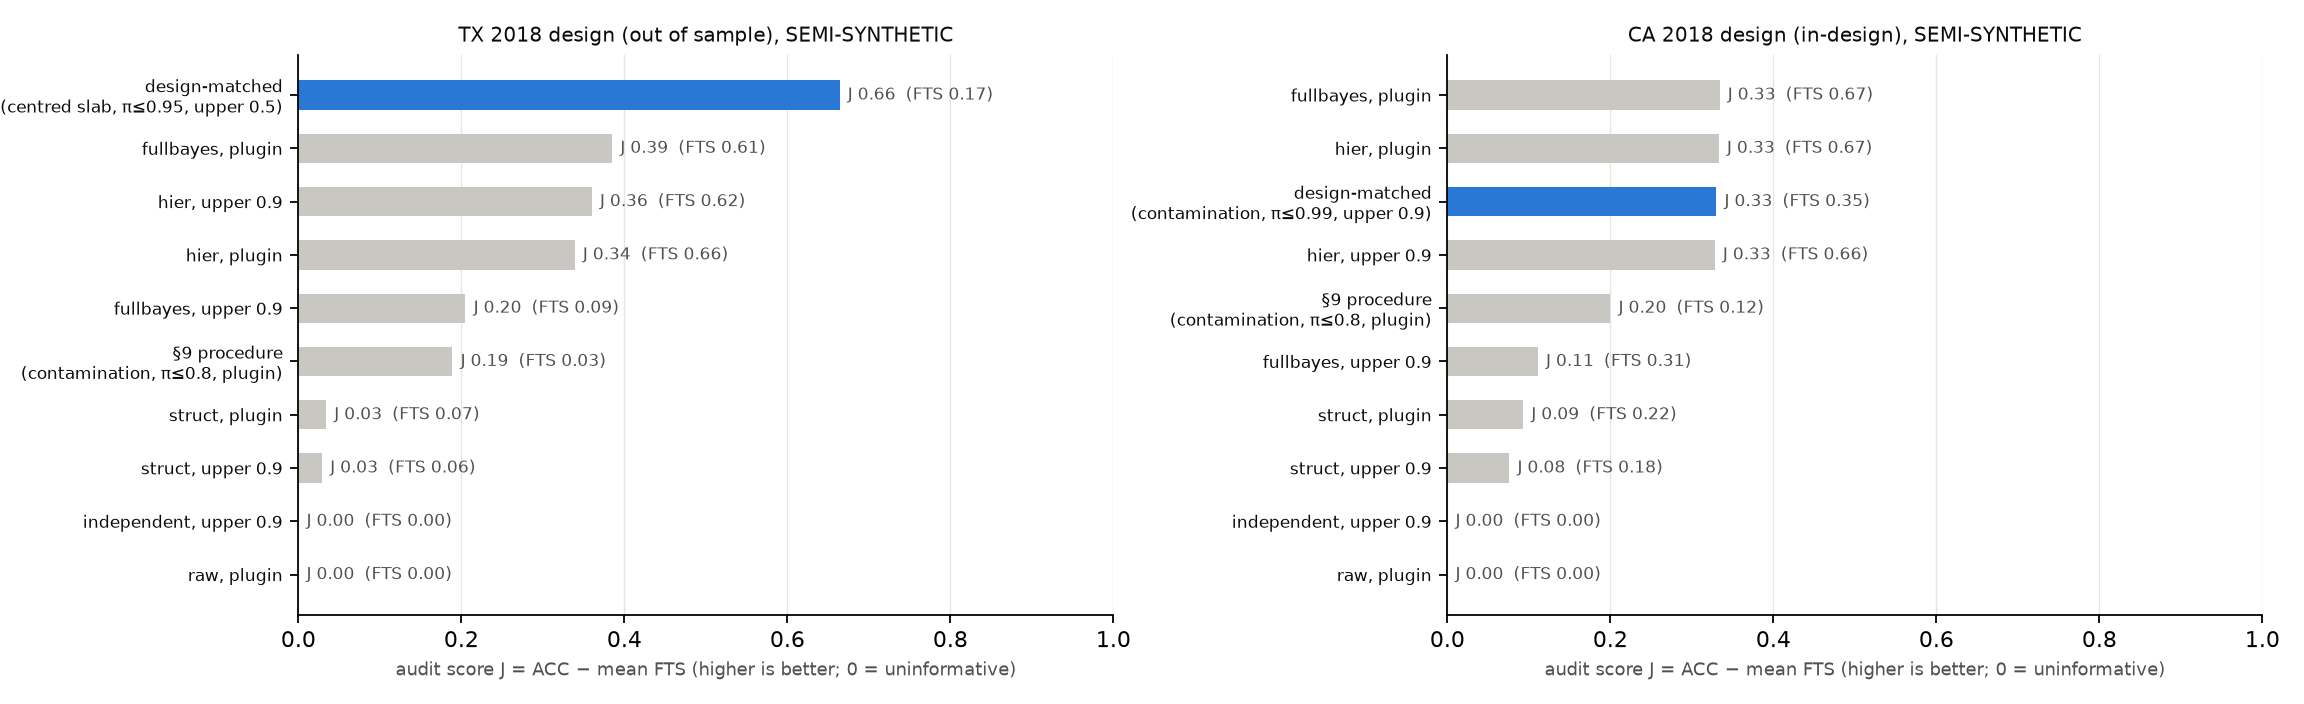
\includegraphics[width=0.86\linewidth]{v2_audit_score}\\[-2pt]
{\tiny Audit score $J$ = ACC $-$ mean FTS on the Texas (left, out of sample) and California (right, pilot) designs.}
\begin{itemize}\footnotesize
\item \textbf{Ablation, no design matching:} fair-world acceptance 0.83 on invented sizes $\to$ 0.32 (CA) and 0.22 (TX);
  90\% of false alarms come from groups with $<10$ positives. \textbf{Same-data certification:} 10/10 claims, all false.
\item \textbf{Robustness:} EB upper 0.9 certifies 98\% of worlds with one hidden 20-positive deficit; a disability
  main-effect deficit is caught by every audit. \textbf{Uncertainty:} bootstrap = evaluation, 5 refits = training
  (mixed signs), simulation = scenario.
\item \textbf{Failure case:} on the CA design $J$ ties ($-0.004$ [$-0.057$, 0.046]); no rule is fair on test (min gap
  0.227); the preregistered real-gap comparison is inconclusive (Holm $p=0.736$).
\end{itemize}
\end{frame}

% Slide 10: 60 seconds.
\begin{frame}{Conclusion and reproducibility}
\begin{itemize}
\item \textbf{Conclusion:} pooling masks isolated small-group deficits, and pooled validation-time claims failed on test
  in every case (H1). Design-matched calibration with held-out certification gives the best audit score out of
  sample on Texas ($J=0.664$ vs at most 0.385) and withheld every false real-data claim.
\item \textbf{Limits and ethics:} simulation evidence comes from one generator family; zero held-out claims shows
  abstention, not sensitivity; the label is not need; no stakeholder set $\epsilon$. Do not call any rule here fair.
\item \textbf{Reproduce:} \url{\RepoURL}, tag \texttt{\SubmitTag};
  \texttt{jupyter nbconvert -{}-execute -{}-inplace Problem8\_Intersectional\_Fairness.ipynb} (about 30 min, 1 CPU).
\item \textbf{\StudentA:} question, literature, data, BN and exact inference, Texas H1 test; cross-checked the audits and $J$.
\item \textbf{\StudentB:} audit models, simulations, threshold selection, bootstrap, design-matched/held-out audit (H2);
  cross-checked splits, labels and inference.
\end{itemize}
\end{frame}

\appendix
\begin{frame}{Backup: mandatory evidence and references}
\scriptsize
\begin{tabularx}{\linewidth}{@{}ll>{\raggedright\arraybackslash}X@{}}\toprule
Requirement & Notebook & Status / artefact\\\midrule
VE vs clique tree, normalisation, CI & \S3.1 & complete; max error $3.3\times10^{-16}$\\
E1 single vs intersectional & \S5 & complete; \texttt{exp1\_single\_two\_three\_way.csv}\\
E2 minority thinning & \S10 & complete; 4 levels $\times$ 5 seeds, \texttt{selection\_all.csv}\\
E3 empirical vs independent vs pooled & \S7 & complete; \texttt{exp3\_estimates\_real.csv}\\
E4 homogeneous vs exceptional worlds & \S8, \S9.2 & complete; \texttt{sim\_main\_summary}, \texttt{semisynthetic\_*}\\
E5 ordinary vs uncertainty-aware selection & \S10 & complete; capacity matched (test 0.292--0.305)\\
Ablations: no / complete pooling, mean vs quantile & \S8, \S10 & complete\\
Robustness: priors, prevalence, $\epsilon$, 2nd state & \S9.1, \S12, \S14 & complete; TX replication\\
Bootstrap $\ge$1000, Holm, $\ge$5 seeds & \S11 & complete; \texttt{confirmatory\_bootstrap.csv}\\
H1 / H2a--c & \S14.1, \S15 & supported; \texttt{h1\_texas\_test}, \texttt{v2\_*}\\\bottomrule
\end{tabularx}\\[4pt]
Full matrix: \texttt{docs/requirements\_matrix.md}. References: Foulds et al.\ SDM 2020; Herlihy et al.\ FAccT 2024;
Kearns et al.\ ICML 2018; Berger \& Berliner, Ann.\ Stat.\ 1986; Ding et al.\ NeurIPS 2021; Cotter et al.\ ICML 2019
(19 in \texttt{writeup/references.tex}).
\end{frame}

\begin{frame}{Backup: inference and statistical validation}
\small
\begin{itemize}
\item \textbf{Factors:} scope and shape validated on construction; evidence reduces by slicing, hidden variables are summed;
  final table normalised. CPT rows sum to 1 ($\alpha=1$ keeps every entry positive).
\item \textbf{Exact inference:} 6-node sub-network, 200 masked-evidence cases: our VE (2 orders), pgmpy VE, clique tree,
  enumeration agree to $3.3\times10^{-16}$. The full-BN fast scorer equals general VE on observed rows.
\item \textbf{Independence:} for each $y$, $P(\text{SEX},\text{AGEP},\text{DIS}\mid y)=P(\text{SEX}\mid y)P(\text{AGEP},\text{DIS}\mid y)$.
\item \textbf{\texttt{struct} audit:} quadrature vs fine grid $9.6\times10^{-11}$; analytic vs numeric gradient $2.0\times10^{-6}$;
  90\% coverage 0.665 fitted vs 0.905 oracle ($\hat\tau$ 0.18 vs true 0.30).
\item \textbf{Denominators:} positives per group 1--5,499 on validation; groups with $<30$ positives flagged exploratory;
  zero-positive groups have undefined TPR.
\item \textbf{Bootstrap:} Poisson(1) weight per household, shared by both arms; percentile CI; Holm over
  \{proposed vs hier plug-in, proposed vs raw plug-in\}: $p_{\text{Holm}}=1.0$, $0.736$.
\end{itemize}
\end{frame}

\begin{frame}{Backup: demonstration and individual defence}
\small
\begin{itemize}
\item \textbf{Live demo (about 15 s):} \texttt{python writeup/make\_tables.py} regenerates every table and the
  paired $\Delta J$ intervals from \texttt{results/}.\\ Expected line: \texttt{TX \dots{} fullbayes $\cdot$ plugin \dots{} 0.279 0.235 0.322}.
\item \textbf{Full regeneration:} execute the notebook (about 30 min, 1 CPU core, downloads 435 MB of ACS data).
\item \textbf{Saved fallback trace:} \texttt{demo/saved\_trace.txt} (inference check, H1 verdict, H2 scores).
\item \textbf{Trace an inference:} a factor with axes $(B,A)$, shape $(3,2)$, times $(B,C)$, shape $(3,4)$, broadcasts to $(2,3,4)$;
  summing $B$ removes its axis; normalising gives $P(\cdot\mid e)$.
\item \textbf{Justify fairness:} TPR range, because the harm is unreached people who need outreach; $\epsilon=0.10$ is a
  value judgement tested at 0.05 and 0.15.
\item \textbf{Critique a claim:} zero held-out false claims follows from zero claims; it shows abstention, not that the
  procedure would certify a really fair rule.
\end{itemize}
\end{frame}
\end{document}
